\chapter{Control system}\label{chap:control_system}
This chapter concerns implementation of a regulator for the pan tilt system. The goal of such systems is that it should increase the performance of the system itself when regulating on stable systems, otherwise when regulating on unstable systems it should be able to stabilise the system. In the dynamics chapter it was concluded that a decoupled model of the system is sufficient and therefore a regulator for pan part and a regulator for the tilt part can be designed individually. 

\section{Design}
SISO\footnote{Single input, single output}-control systems can be sketched the following way:
\begin{figure}[htb]
	\centering
	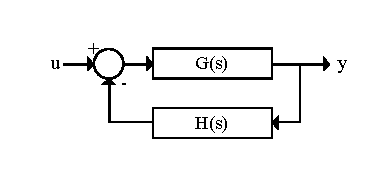
\includegraphics[width=\textwidth,trim=0 0 0 0]{graphics/control_sketch.pdf} %trim=l b r t (can cut off from every side)
	\caption{This figure illustrates a sketch of a general control system.}
	\label{fig:control_sketch}			% figure labels are of the form \label{fig:*}
\end{figure}
Figure \ref{fig:control_sketch} show a system with a feedback loop, $G(s)$ is theplant and $H(s)$ is the regulator. When designing a regulator ($H(s)$) is derived and since the system is SISO, a PID regulator can be designed.

\subsection{PID parameters}
A PID regulator can be expressed in the following way:
\begin{equation}
	h(t) = K_p e(t) + K_i \int\limits_0^t e(\tau) d\tau + K_d \frac{de(t)}{dt}
\end{equation}
where $K_p$, $K_i$, and $K_d$ are constants for the proportional, integral, and differential term in the equation. Applying LaPlace-transform leads to:
\begin{equation}
	H(s) = E(s)(K_p + \frac{K_i}{s} + K_d s)
\end{equation}
Though various methods are available for deriving the optimal parameters, the approach chosen here is to do a mathematical simulation of the system. Since the transfer functions have already been derived, a Simulink model can be developed. Since the system is decoupled, it can be represented as shown in \ref{fig:control_sketch}
\begin{figure}[htb]
	\centering
	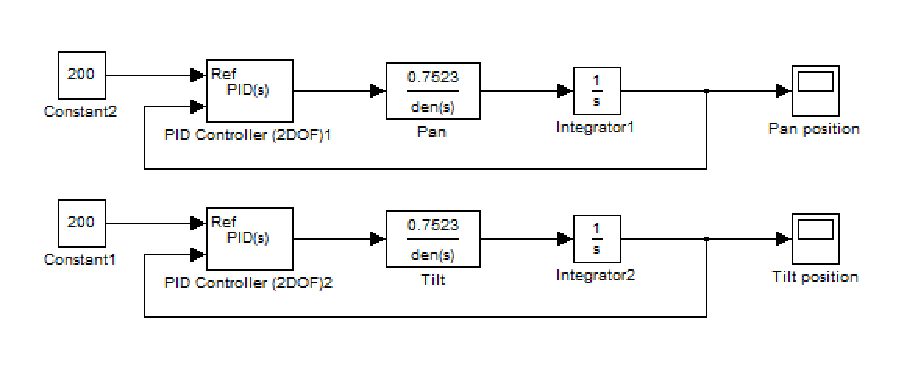
\includegraphics[width=\textwidth,trim=0 0 0 0]{graphics/Simulink.pdf} %trim=l b r t (can cut off from every side)
	\caption{This figure illustrates the simulink model.}
	\label{fig:control_sketch}			% figure labels are of the form \label{fig:*}
\end{figure}
The top system represent the pan part of the system, while the lower part represent the tilt.

\section{Simulation}
The goal of the simulation is to find the values providing the most dynamic system, while still remaining stable and robust. To obtain a first guess of the P-term, the root locus method is applied. The root locus plot can be seen in \ref{fig:rlocus_plot}. Aiming to minimize the energy needed to move the system, equal magnitudes of real and imaginary parts are chosen, leading to the base gain denoted in \ref{tab:gain_values}.

\begin{figure}[htb]
	\centering
	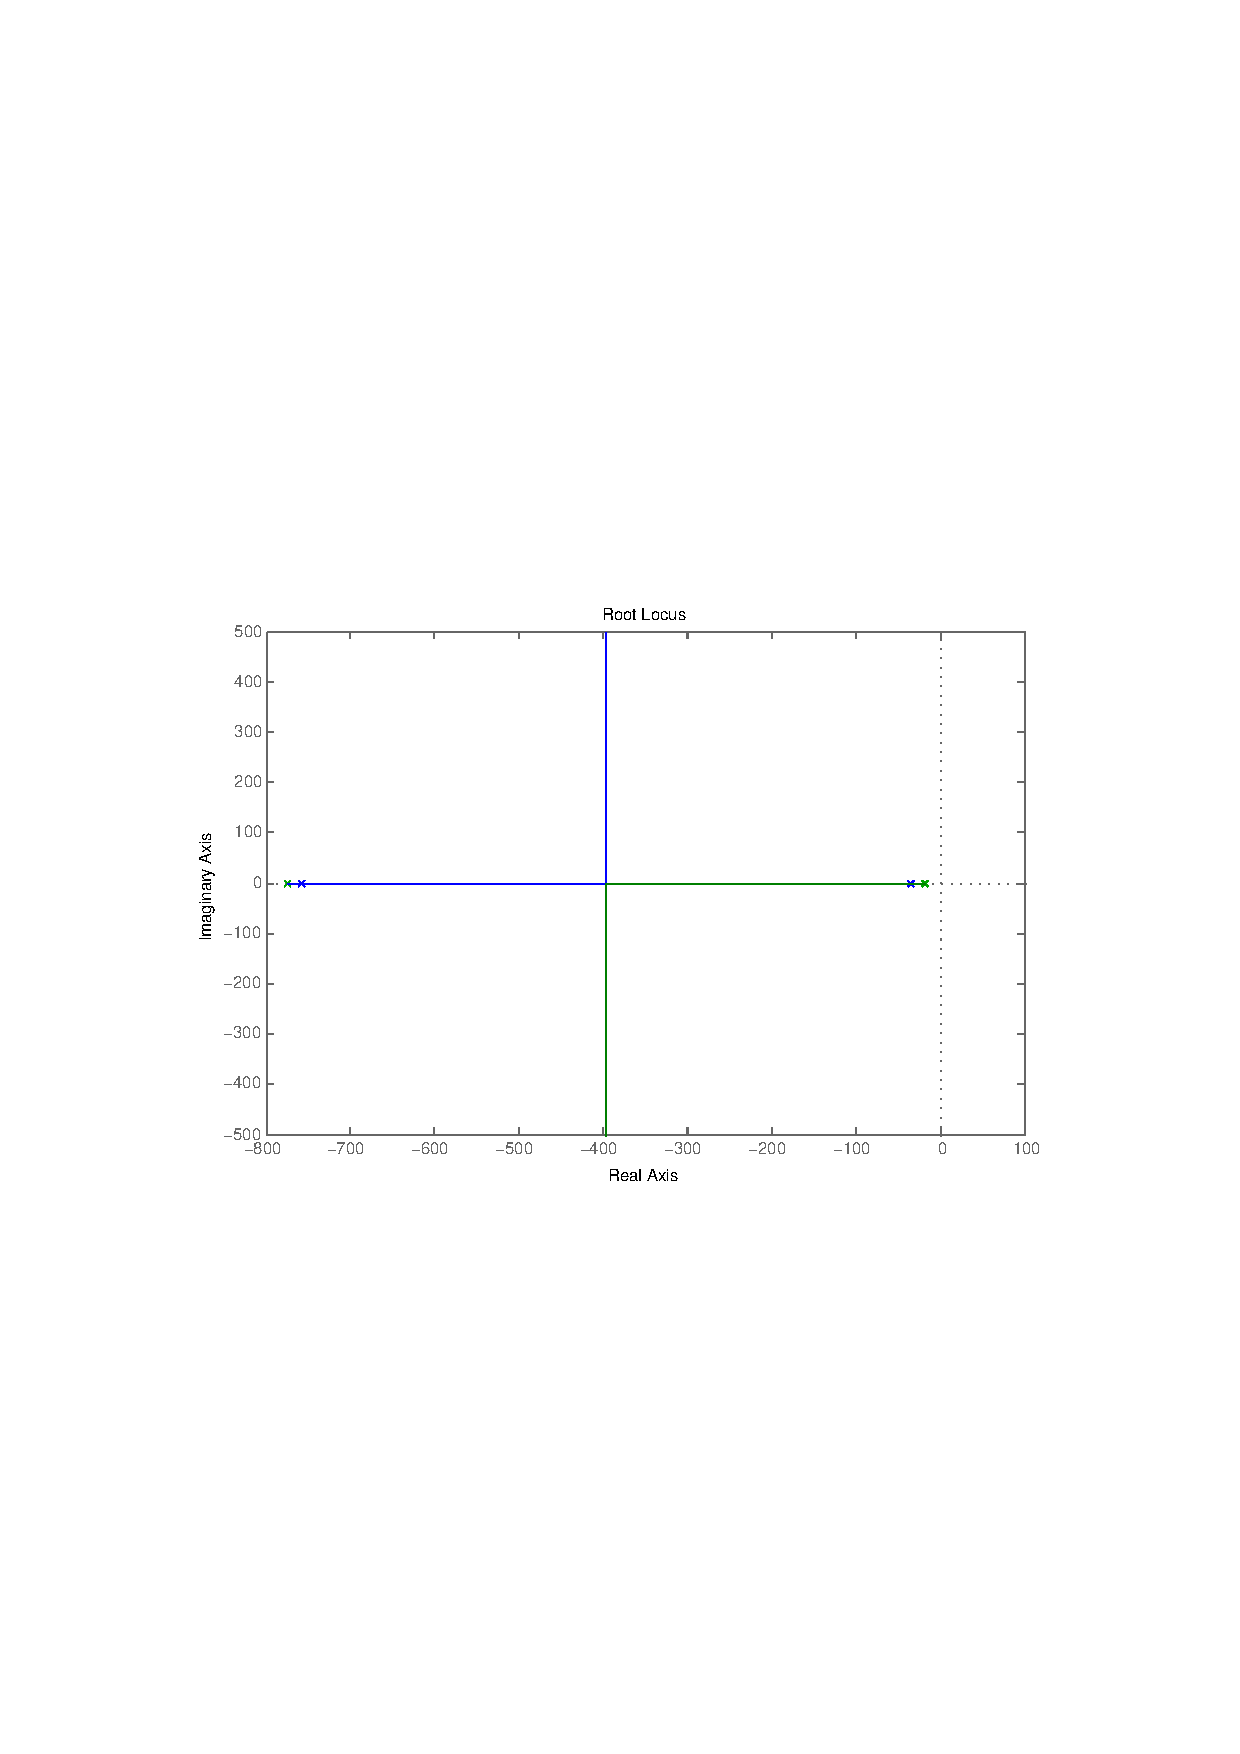
\includegraphics[width=\textwidth,trim=0 270 0 270]{graphics/rlocus_plot.pdf} %trim=l b r t (can cut off from every side)
	\caption{Shows the root locus plot the pan and tilt systems.}
	\label{fig:rlocus_plot}			% figure labels are of the form \label{fig:*}
\end{figure}

The simulation is run with various parameters to find the range of values in \ref{tab:gain_vaues}. \ref{chosen_plot} shows a plot of the chosen values, where the system settles within five seconds.

\begin{table}[htb]				
	\begin{center}
	\begin{tabular}{l|c|c|c|c}			
	Term & Base & Maximum & Auto tune & Chosen \\			
	\hline												
P-gain pan& 6 & 450 & 37.2 & 30\\
P-gain tilt& 6 & 450 & 39.2 & 30\\
I-gain pan& 0 & 250* & 19.9  & 20\\
I-gain tilt& 0 & 350* & 20.43 & 20\\
D-gain pan& 0 & 70** & 1.9 & 1\\
D-gain tilt& 0 & 100** & 0.7 & 1\\
	\end{tabular}
	\end{center}
	\caption{Gain values derived from simulation. *@P=30 and D=0. **@P=30 and I=0}				
	\label{tab:gain_values}			
\end{table}

\begin{figure}[htb]
	\centering
	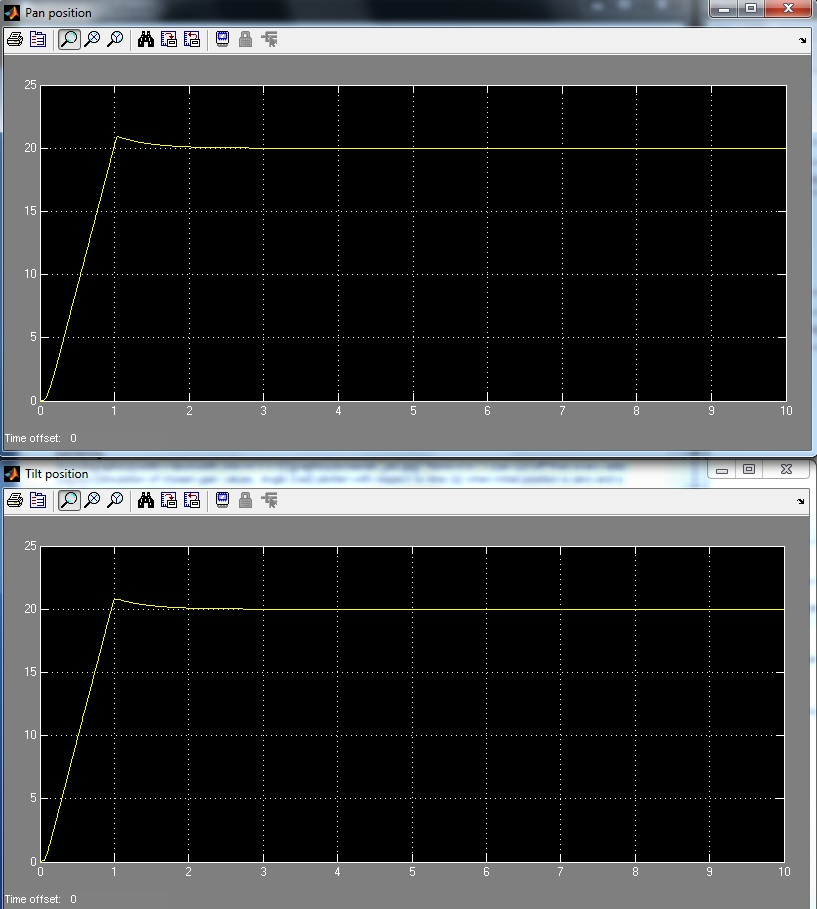
\includegraphics[width=\textwidth,trim=0 0 0 0]{graphics/screensh_pid.jpg} %trim=l b r t (can cut off from every side)
	\caption{Simulation of chosen gain values. Angle [rad] plottet with respect to time [s] when initial position is zero and a setpoint of 20 is given as step.}
	\label{fig:chosen_plot}			% figure labels are of the form \label{fig:*}
\end{figure}

\section{Implementation}
The control algorithm is implemented in the control task. All parameters are provided from the parameter server but are cast as single precision floating point values for exact calculations.

When run the control task saves the value of the tick counter and when finished, it uses the FreeRTOS \texttt{vTaskDelayUntil} API to calculate when to unblock. As a starting point the control task runs at one hundred hertz frequency.

For calculating the error, a common format is needed. The parameter server holds the setpoint in degrees and the actual position in ticks. To be able to use some intuition about the control algorithm, degrees are chosen and the position in degrees is calculated by using a ticks to degrees factor calculated from knowing the gears and the number of ticks per motor round.
\begin{equation}
1 \ tilt \ revolution \ * 30:1 \ planet \ gear \ * 3:1 \ belt \ gear = 90 \ motor \ rounds
\end{equation}
\begin{equation}
 90 \ motor \ rounds * 12 \ ticks/round = 1080 \ ticks/tilt \ revolution
\end{equation}
This number is then used to calculate the ratio of degrees to ticks, keeping in mind that degrees have an implicit decimal:

\begin{equation}
\frac{360 \ deg \times 10}{1080 \ ticks} = 3.34\ deg/tick 
\end{equation}

The error is then calculated as the difference between setpoint and actual position and is thus a signed value in degrees.

\subsection{Implementing proportionality gain}
A first guess for the proportionality gain is to make an error of ten degrees resemble a ten percent PWM signal and an error of a hundred degrees resemble full speed. The PWM signal range from five thousand, where the motor barely moves up to the maximum of a 16 bit signed, where the motor runs full speed.
\begin{equation}
2^{15} = 32.767 \Rightarrow 
32.767 - 5000 = 27.767 \Rightarrow 
1 \% = \frac{27.767}{100} \approx  277
	\label{eq:PWM}
\end{equation}
 Therefore the first guess is calculated:
\begin{equation}
10x = 5000 + (10 * 270) => x = \frac{7770}{10} \approx  8
	\label{eq:P-term}
\end{equation}
This in within the range found from simulation so the system should remain stable. Since it is possible to get PWM values out of the range specified in (REFERENCE!), a maximum function is implemented, so that absolute values out of range are corrected to the maximum value.

Since PWM values below a certain minimum does not make the motor move, a bias is added so that non-zero values are added with the bias value. A tresholdl is implemented so that values inside the +/- treshold area is zeroed before the bias is added. If this was not done even the smallest error would be biased.

\subsection{Adjusting the P-gain}
Testing of the system confirms that the proportionality factor works well and the system tracks the given position. Testing on only the tilt part of the system shows, that at proportionality gain values above 22, the system becomes unstable. The maximum stable value is at 16 but this makes the system less robust, resulting in instability when the system is stressed, so a value around 10 seems fit.

\subsection{Integrator}
Since the error grows smaller as the goal is approached, movement almost halt when approaching the goal area, making the system less accurate and slower. Therefore an integration term is implemented by adding the errror to the integration value on each run. Thereby in the situation where the error is too small to make the system move, the integration term will rise and thus add to the input. 

Normally an integration would mean the product of the value and the time since last sample, but presuming that this time is nearly constant it can be calculated as part of the I-term. 

To keep the integration from going to infinity, an anti wind up filter is implemented. Wind up happens for example when the system is stopped while not at the setpoint and the integration reaches high values that has to be overcome when the system resumes.

\subsection{Adjusting the I-gain}
Testing was done with a fixed P-gain of ten and integrator windup max at ten thousand. As a first guess the I-gain was set to 1 which made the system unstable. Additional testing showed that values a hundred times less were more appropriate. The system becomes unstable around 0.1 and a value of 0.05 was chosen.

Testing showed that the tracking ability of the system had substantially increased and the speed has increased especially when close to the goal. Only after changing setpoint, the system seems slow. This suggest implementing a differentiator term.

\subsection{differentiator}
By saving the error at each entry it is possible to calculate the change in the error. This term will be particularly large just after changing the setpoint, and can thus help improve the acceleration.

The actual derivative would be the change in value over the time since last entry, but as for the integrator, this can be omitted presuming that it is constant.

In a faulty system it could be considered implementing a maximum on the differentiator to prevent wrong or noisy measurements of having too much impact on the system. As a start this is not implemented as to not solve the problem until it arise.

\subsection{Adjusting the D-gain}
Testing was done with a fixed P-gain of ten, I-gain of 0.05 with anti-windup at ten thousand. As a first guess the D-gain was set to
